\documentclass[a4paper]{article}

\usepackage[utf8]{inputenc}
\usepackage[margin=1in]{geometry}
\usepackage[square,numbers]{natbib}
\usepackage{hyperref}
\usepackage{listings}
\usepackage{bussproofs}
\usepackage{fancyvrb}
\usepackage{booktabs}
\usepackage{subcaption}
\usepackage{todonotes}
\usepackage{xcolor}
\usepackage{tabularx}
\usepackage{comment}
\usepackage{mathtools}
\usepackage{csquotes}
\usepackage{mathpartir}
\usepackage{stmaryrd}
\usepackage{microtype}
\usepackage{standalone}
\usepackage{import}
\usepackage{multicol}
\usepackage{soul}
\usepackage[capitalize,nameinlink,noabbrev]{cleveref}
\usepackage[inline]{enumitem}
\usepackage{cmll}
\usepackage{amsfonts,amsmath,stmaryrd,amsthm,amssymb}
\usepackage[T1]{fontenc}
\usepackage[all]{xy}
\usepackage{xspace}
\usepackage{latexsym}
\usepackage{bbm}
\usepackage{mathrsfs}
\usepackage{graphicx}
\usepackage{color}
\usepackage[all]{xy}
\usepackage{stackrel}
\usepackage{iris}
\usepackage{syn}
\usepackage{macro}

\usepackage{tikz}
\usepackage{tikz-cd}
\usetikzlibrary{automata, positioning, arrows}

\tikzset{
  ->, % makes the edges directed
  node distance=3cm, % specifies the minimum distance between two nodes. Change if necessary.
  every state/.style={thick, fill=gray!10}, % sets the properties for each ’state’ node
  initial text=$ $, % sets the text that appears on the start arrow
}

\setlength{\columnsep}{0pc}

\definecolor{dkgreen}{rgb}{0,0.6,0}
\definecolor{ltblue}{rgb}{0,0.4,0.4}
\definecolor{dkviolet}{rgb}{0.3,0,0.5}

\newtheoremstyle{break}
  {\topsep}{\topsep}%
  {\itshape}{}%
  {\bfseries}{}%
  {\newline}{}%

\lstset{basicstyle=\ttfamily}

\newcommand{\citets}[1]{\citeauthor{#1}'s~[\citeyear{#1}]}

\bibliographystyle{abbrvnat}

\newtheorem{theorem}{Theorem}[section]
\newtheorem{corollary}{Corollary}[theorem]

\newtheorem{lemma}[theorem]{Lemma}

\theoremstyle{break}
\newtheorem{definition}{Definition}[section]

\theoremstyle{remark}
\newtheorem*{remark}{Remark}

\title{call/cc meets guarded interaction trees (note)}
\author{}
\date{\today}

\begin{document}

\maketitle

\noindent

\section*{Preface}
Non-trivial control flow operations, such as call/cc, provide immense
control over program execution but also make formal reasoning about
programming languages supporting it more complicated. In this note, we
provide denotational semantics of call/cc, defined in guarded
interaction trees, and prove that this semantics reflects the expected
operational behaviour.
\label{global:sec:preface}

\tableofcontents

\clearpage

\section{Introduction}
\label{global:sec:intro}
In this note, we investigate the extension to Guarded Interaction Trees to
support context-dependent effects (e.g., call/cc and throw).

This note is divided into a few sections. In~\cref{global:sec:gitree} we
recall definition and relevant properties of guarded interaction
trees. In~\cref{global:sec:lang} we describe the calculus with callcc,
which we study in this note. In~\cref{global:sec:reifier} we describe
modifications to guarded interaction trees required to interpret
context-dependent effects. In~\cref{global:sec:sem} we provide a
denotational model for a language with callcc in guarded interaction
trees with modifications and prove soundness and adequacy of the
model.

%%% Local Variables:
%%% mode: latex
%%% TeX-master: "../main"
%%% TeX-master: "../main"
%%% End:


\section{Guarded interaction trees}
\label{global:sec:gitree}
Guarded Interaction trees (\gitrees) are constructed as a guarded
recursive type parameterized over two input types: $E$ that provides
an effect signature, which specifies effects that can occur, and their
arity. $A$ specifies a ground type that allows addition of new
primitive values. The type has five constructors: $\Rret$ --- wraps
ground type expressions, $\Fun$ extends the domain to contain
functions, $\Err$ constructor, $\Tau$ constructor that makes \gitrees
into guarded domain, and $\Vis$ that accepts a function from inputs of
some effect (that can involve \gitrees themselves, which allow us to
represent higher-order effects), a function from outputs of the same
effect to gitrees, which represents continuations of effects.

\gitrees admit an operational semantics given reifiers for all effects
in the signature. A reifier of an effect $i$ is a function of type
shown in~\cref{fig:reifier_sig}. Assuming we have such reifiers for
all effects, we write a function $\reify : \IT \times \stateO \to \IT
\times \stateO$ that satisfies the equations in~\cref{fig:reify_def}.
Note that reifiers don't take continuation into account. Now we can
define a step to be either removing a single $\Tick$ (where $\Tick
\eqdef \Tau \circ \Next$), or reification of the head effect.

Let us now define a class of homomorphic functions, formally defined
in~\cref{fig:hom}, to be functions that act as identities on errors,
and preserve $\Tick$ and $\Vis$ constructors.

Now, given $\istep$ representing operational semantics of \gitrees,
and homomorphic functions, representing context of \gitrees. We can
define program logic for a language of \gitrees, including important
wp-bind and wp-reify rules (\cref{fig:wp_rules}), which allow to
modular reasoning about \gitrees and effects respectfully.

\begin{figure}[t]
  \begin{align*}
    \mathsf{guarded\ type}\ \IT_E(A) &{}= \Rret : A \to \IT_E\\
                                     &\ \ALT \Fun : \latert (\IT_E(A) \to \IT_E(A)) \to \IT_E(A)\\
                                     &\ \ALT \Err : \Error \to \IT_E(A)\\
                                     &\ \ALT \Tau : \latert \IT_E(A) \to \IT_E(A) \\
                                     &\ \ALT \Vis : \prod_{\idx \in \mathtt{I}} \big( \Ins_{\idx}(\latert \IT_E(A)) \times (\Outs_{\idx}(\latert \IT_E(A)) \to \latert \IT_E(A))\big) \to \IT_E(A)
  \end{align*}

  \caption{Guarded datatype of interaction trees.}
  \label{fig:gitrees_def}
\end{figure}

\begin{figure}
  \[
    r : \prod_{\idx \in E} \Ins_{\idx}(\latert \IT_E) \times \stateO \to \optionO(\Outs_{\idx}(\latert\IT_E) \times \stateO).
  \]
  \caption{Signature of reifiers.}
  \label{fig:reifier_sig}
\end{figure}

\begin{figure}
  \begin{mathpar}
    \infer
    {r_i(x,\sigma) = \Some(y, \sigma') \and k\ y = \Next(\beta)}
    {\reify(\Vis_i(x, k), \sigma) = (\Tick(\beta), \sigma')}
    \and
    \infer
    {r_i(x,\sigma) = \None}
    {\reify(\Vis_i(x, k), \sigma) = (\Err(\RunTime), \sigma)}
  \end{mathpar}
  \caption{Reification definition.}
  \label{fig:reify_def}
\end{figure}

\begin{figure}
  \[
    (\alpha,\sigma) \istep (\beta,\sigma') \eqdef
    \big(\alpha = \Tick(\beta) \wedge \sigma = \sigma' \big)
    \vee \big(\Exists i\,x\,k. \alpha = \Vis_i(x,k)
    \wedge \reify(\alpha,\sigma) = (\Tick(\beta),\sigma')\big)
  \]
  \caption{Operational semantics of Guarded interaction trees.}
  \label{fig:opsem_gitrees}
\end{figure}

\begin{figure}
  \begin{itemize}
  \item $f(\Err(e)) = \Err(e)$;
  \item $f(\Tick(\alpha)) = \Tick(f(\alpha))$;
  \item $f(\Vis_i(x,k)) = \Vis_i(x, \latert f \circ k)$
  \end{itemize}
  \caption{Homomorphisms}
  \label{fig:hom}
\end{figure}

\begin{figure}
  \begin{mathpar}
    \inferrule[wp-reify]
    {\hasstate(\sigma) \and
      \reify(\Vis_i(x,k), \sigma) = (\Tick(\beta), \sigma')
      \and
      \later\big(\hasstate(\sigma') \wand \wpre{\beta}{\Phi} \big)}
    {\wpre{\Vis_i(x, k)}{\Phi}}
    \and
    \inferrule[wp-hom]
    {f \in \Hom \and \wpre{\alpha}{\Ret \beta_v. \wpre{f(\beta_v)}{\Phi}}}
    {\wpre{f(\alpha)}{\Phi}}
  \end{mathpar}
  \caption{Selected weakest precondition rules.}
  \label{fig:wp_rules}
\end{figure}

%%% Local Variables:
%%% mode: latex
%%% TeX-master: "../main"
%%% End:


\section{Language}
\label{global:sec:lang}
In this section we describe our target language, $\iocclang$.

$\iocclang$, presented in~\cref{fig:syn_lang}, is a lambda calculus
with recursive functions, primitive natural numbers and operations on
them, input/output operations, call/cc, and throw. In addition, it has
first-order evaluation contexts.

$\callcc{\var}{\expr}$ stands for a computation that takes the current
evaluation context (i.e., the evaluation context, where the term is
being evaluated), and binds it with $\var$ in $\expr$.
$\throw{\expr_1}{\expr_2}$ takes two arguments, the first being any
expression, and the second being an evaluation context.

$\iocclang$ has a type system, shown in~\cref{fig:stat_sem_lang}, that
includes natural numbers type, function type and a type or
continuations that accept expressions of type $\tau$, represented by
$\tcont{\tau}$.

Operational semantics on this language is presented
in~\cref{fig:dyn_sem_lang,fig:dyn_global_sem_lang}. It is separated
into two relations. The first relation is for local reductions of
primitive expressions, while the second one accounts for steps lifted
to complete programs. Both relations are parameterized over
configurations that contain expressions and states, where states are
two lists of natural numbers, representing input and output tapes
respectfully. In addition, the local relation is parameterized over
evaluation context, which allows $\callcc{\var}{\expr}$ to capture the
whole evaluation context.

To give an interpretation of this language we need to provide an
effect signature, and interpretations for all effectful computations
that it exhibits.

Let us start by the effect signature, shown
in~\cref{fig:eff_sig_lang}. The language contains four different
effects: $\mathtt{input}$, $\mathtt{output}$, $\mathtt{callcc}$,
$\mathtt{throw}$. $\mathtt{input}$ doesn't require any arguments and
yields back a natural number, so its input has type $\Tunit$, and its
output has type $\Tnat$. Similar reasoning is also applicable to
$\mathtt{output}$. $\mathtt{callcc}$ and $\mathtt{throw}$, on the
other hand, require higher-order arguments. The behavior of
$\callcc{\var}{\expr}$ is determined by its body that binds a
continuation and utilizes it, so a natural approach is to require
that its input is of type of its body, $(\latert X \rightarrow \latert
X) \rightarrow \latert X$. Moreover, the result of
$\callcc{\var}{\expr}$ is determined by its body, so its output is
$\latert X$. $\throw{\expr_1}{\expr_2}$ requires an expression and a
continuation, which are represented respectfully as $\latert X$ and
$\latert (X \rightarrow X)$. As for the output,
$\throw{\expr_1}{\expr_2}$ discard the current continuation, hence it
is safe to assume that its continuation is a unique function out of
the empty type.

We write $\INPUT$, $\OUTPUT(n)$, $\callccGT(f)$, and $\throwGT(e)$ for
the \gitrees defined in~\cref{fig:io_constructors}.

\begin{figure}
  \begin{grammar}
    \text{types} & \tau & \tnat \mid \tarr{\tau_1}{\tau_2} \mid \tcont{\tau} \\
    \text{expressions} & \expr & \val \mid \var \mid \eapp{\expr_1}{\expr_2} \mid \natop{\expr_1}{\expr_2} \mid \Input \mid \Output \expr \mid \If \expr_1 then \expr_2 \Else \expr_3 \\
    \GrmContinue & \mid \callcc{\var}{\expr} \mid \throw{\expr_1}{\expr_2} \\
    \text{values} & \val & n \mid \Rec f \var = \expr \mid \cont{K} \\
    \text{evaluation contexts} & K & \emptyK \mid \Output K \mid \If K then \expr_1 \Else \expr_2 \mid \eapp{K}{\val} \mid \eapp{\expr}{K} \mid \natop{\expr}{K} \mid \natop{K}{\val} \\
    \GrmContinue & \mid \throw{K}{\expr} \mid \throw{\val}{K}
  \end{grammar}
  \caption{Syntax of $\iocclang$.}
  \label{fig:syn_lang}
\end{figure}

\begin{figure}
  \begin{mathpar}
    \inferrule{\var \col \tau \in \Gamma}{\typeA{\Gamma}{\var}{\tau}}
    \and
    \inferrule{\typeA{\Gamma, f \col \tarr{\tau_1}{\tau_2}, \var \col \tau_1}{\expr}{\tau_2}}{\typeA{\Gamma}{\Rec f \var = \expr}{\tarr{\tau_1}{\tau_2}}}
    \and
    \inferrule{\typeA{\Gamma}{\expr_1}{\tarr{\tau_1}{\tau_2}} \\ \typeA{\Gamma}{\expr_2}{\tau_1}}{\typeA{\Gamma}{\eapp{\expr_1}{\expr_2}}{\tau_2}}
    \and
    \inferrule{}{\typeA{\Gamma}{\Input}{\tnat}}
    \and
    \inferrule{\typeA{\Gamma}{\expr_1}{\tnat} \\ \typeA{\Gamma}{\expr_2}{\tau} \\ \typeA{\Gamma}{\expr_3}{\tau}}{\typeA{\Gamma}{\If \expr_1 then \expr_2 \Else \expr_3}{\tau}}
    \and
    \inferrule{\typeA{\Gamma}{\expr}{\tnat}}{\typeA{\Gamma}{\Output \expr}{\tnat}}
    \and
    \inferrule{}{\typeA{\Gamma}{n}{\tnat}}
    \and
    \inferrule{\typeA{\Gamma}{\expr_1}{\tnat} \\ \typeA{\Gamma}{\expr_2}{\tnat}}{\typeA{\Gamma}{\natop{\expr_1}{\expr_2}}{\tnat}}
    \and
    \inferrule{\typeA{\Gamma, \var \col \cont{\tau}}{\expr}{\tau}}{\typeA{\Gamma}{\callcc{\var}{\expr}}{\tau}}
    \and
    \inferrule{\typeA{\Gamma}{\expr_1}{\tau} \\ \typeA{\Gamma}{\expr_2}{\cont{\tau}}}{\typeA{\Gamma}{\throw{\expr_1}{\expr_2}}{\tau'}}
  \end{mathpar}
  \caption{Static semantics $\iocclang$.}
  \label{fig:stat_sem_lang}
\end{figure}

\begin{figure}
  \begin{mathpar}
    \inferrule{}{\contrA{\eapp{\Rec f \var = \expr}{\val}, \sigma}{\subst{\subst{\expr}{f}{\Rec f \var = \expr}}{\var}{\val}, \sigma}{K}}
    \and
    \inferrule{}{\contrA{\If 0 then \expr_1 \Else \expr_2, \sigma}{\expr_2, \sigma}{K}}
    \and
    \inferrule{0 < n}{\contrA{\If n then \expr_1 \Else \expr_2, \sigma}{\expr_1, \sigma}{K}}
    \and
    \inferrule{\natop{n_1}{n_2} = n_3}{\contrA{\natop{n_1}{n_2}, \sigma}{n_3, \sigma}{K}}
    \and
    \inferrule{}{\contrA{\Input, (n\overline{n}, \overline{m})}{n, (\overline{n}, \overline{m})}{K}}
    \and
    \inferrule{}{\contrA{\Output m, (\overline{n}, \overline{m})}{0, (\overline{n}, m\overline{m})}{K}}
    \and
    \inferrule{}{\contrA{\callcc{\var}{\expr}, \sigma}{\subst{\expr}{\var}{\cont{K}}, \sigma}{K}}
  \end{mathpar}
  \caption{Dynamic semantics of $\iocclang$ (head-steps).}
  \label{fig:dyn_sem_lang}
\end{figure}

\begin{figure}
  \begin{mathpar}
    \inferrule{}{\contr{\plug{K}{\throw{\val}{\cont{K'}}}, \sigma}{\plug{K'}{\val}, \sigma}}
    \and
    \inferrule{\contrA{\expr_1, \sigma_1}{\expr_2, \sigma_2}{K}}{\contr{\plug{K}{\expr_1}, \sigma_1}{\plug{K}{\expr_2}, \sigma_2}}
  \end{mathpar}
  \caption{Dynamic semantics of $\iocclang$ (global-steps).}
  \label{fig:dyn_global_sem_lang}
\end{figure}

\begin{figure}
  \begin{align*}
    E_{io, callcc} &\eqdef \{\mathtt{input}, \mathtt{output}, \mathtt{callcc}, \mathtt{throw}\} &\\
    \Ins_{\mathtt{input}}(X) &\eqdef \Tunit & \Outs_{\mathtt{input}}(X) &\eqdef \Tnat\\
    \Ins_{\mathtt{output}}(X) &\eqdef \Tnat & \Outs_{\mathtt{ouput}}(X) &\eqdef \Tunit\\
    \Ins_{\mathtt{callcc}}(X) &\eqdef ((\latert X \rightarrow \latert X) \rightarrow \latert X) & \Outs_{\mathtt{callcc}}(X) &\eqdef \latert X \\
    \Ins_{\mathtt{throw}}(X) &\eqdef \latert X \times \latert (X \rightarrow X) & \Outs_{\mathtt{throw}}(X) &\eqdef O
  \end{align*}
  \caption{Effect signature for $\iocclang$.}
  \label{fig:eff_sig_lang}
\end{figure}

\begin{figure}
  \begin{align*}
    \INPUT \eqdef \Vis_{\mathtt{input}}((), \Lam n. \Next(\Rret(\inr(n)))) && \OUTPUT(n) \eqdef \Vis_{\mathtt{output}}(n, \Lam x. \Next (\Rret(\inl(())))) \\
    \callccGT(f) \eqdef \Vis_{\mathtt{callcc}}{(f, \imath)} &&
                                                                                                                              \throwGT(e, f) \eqdef \Vis_{\mathtt{throw}}{(e, f, \mathrm{elim-0})}
  \end{align*}
  \caption{\gitrees for effects}
  \label{fig:io_constructors}
\end{figure}

%%% Local Variables:
%%% mode: latex
%%% TeX-master: "../main"
%%% End:


\section{Reifiers}
\label{global:sec:reifier}
Now, if we want to reason about a language with control operations,
such as $\iocclang$, we have to provide reifiers for its effects.
However, in the current setup, we cannot do that. Consider
$\callccGT(f)$. Before passing results of reification to the current
continuation, it is supposed to take the said continuation, and pass
it to $f$. Analogously, $\throwGT$ is not supposed to return results
of reification at all. With that being said, we cannot define reifiers
for $\callccGT$ and $\throwGT$. A solution to this problem is to make
reifiers accept continuation as an extra parameter, as shown
in~\cref{fig:different_reifiers}.

There is, however, a tradeoff --- the lack of generic bind rule.

\begin{mathpar}
  \inferrule[wp-hom]
  {f \in \Hom \and \wpre{\alpha}{\Ret \beta_v. \wpre{f(\beta_v)}{\Phi}}}
  {\wpre{f(\alpha)}{\Phi}}
\end{mathpar}

The reason for that is the following two lemmas, required to prove that steps can be performed under an arbitrary \gitrees context (i.e., under homomorphic functions).

\begin{lemma}
  \label{lem:hom_istep}
  Let $f$ be a homomorphism.
  Then $(\alpha,\sigma)\istep(\beta,\sigma')$ implies
  $(f(\alpha),\sigma)\istep(f(\beta),\sigma')$.
\end{lemma}
\begin{lemma}
  \label{lem:hom_istep_inv}
  Let $f$ be a homomorphism.
  If $(f(\alpha), \sigma)\istep(\beta',\sigma')$ then either
  \begin{itemize}
  \item $\alpha$ is a \gitree-value, or;
  \item there exists $\beta$ such that
    $(\alpha,\sigma)\istep(\beta,\sigma')$ and $\later(f(\beta) = \beta')$.
  \end{itemize}
\end{lemma}

Consider the second clauses of $\istep$ in both lemmas. By definition
of homomorphic functions, the preserve $\Vis$ constructors by
composition with their continuations. However, we cannot guarantee
that results of reification stay the same with different
continuations.

However, we can recover the bind rule for effect signatures with only
context independent effects, as reifiers for context independent
effects do not depend upon continuations.

Under the proposed modifications, it is possible to define reifiers
for $\callccGT(f)$ and $\throwGT(e)(f)$, as shown
in~\cref{fig:control_reifiers}. Reifiers for $\callccGT(f)$ and
$\throwGT(e)(f)$ are straitforward. $\callccGT(f)$ applies the current
continuation to $f$ `passing` it, and returns the result wrapped in
the current continuation. $\throwGT(e)(f)$ simply applies the second
argument to the first one, and ignores the current continuation
entirely. In addition, we can show the following rules for the
mentioned reifiers.

\begin{lemma}{WP-throw.}
  \label{lem:wp_throw}
  $\sem{\sigma} \ast \later (\sem{\sigma} \wand \wpre{\eapp{f}{x}}{\Phi}) \vdash \wpre{\eapp{\kappa}{(\throwGT(\Next(x))(\Next(f)))}}{\Phi}$
\end{lemma}

\begin{lemma}{WP-callcc.}
  \label{lem:wp_callcc}
  $\sem{\sigma} \ast \later (\sem{\sigma} \wand \wpre{\eapp{\kappa}{(\eapp{f}{\kappa})}}{\Phi}) \vdash \wpre{\eapp{\kappa}{(\callccGT(\Next \circ f))}}{\Phi}$
\end{lemma}

\begin{figure}
  \[
    r : \prod_{\idx \in E} \Ins_{\idx}(\latert \IT_E) \times \stateO \times (\Outs_{\idx}(\latert \IT_E \rightarrow \latert \IT_E)) \to \optionO(\latert \IT_E \times \stateO).
  \]
  \caption{New type for reifiers.}
  \label{fig:different_reifiers}
\end{figure}

\begin{figure}
  \begin{mathpar}
    \infer
    {r_i(x,\sigma,\kappa) = \Some(\beta, \sigma')}
    {\reify(\Vis_i(x, k), \sigma) = (\Tau(\beta), \sigma')}
    \and
    \infer
    {r_i(x,\sigma,\kappa) = \None}
    {\reify(\Vis_i(x, k), \sigma) = (\Err(\RunTime), \sigma)}
  \end{mathpar}
  \caption{New definition of reify function.}
  \label{fig:different_reify}
\end{figure}

\begin{figure}
  \begin{align*}
    r_{\mathtt{input}}((),(n\vec{n},\vec{m}),\kappa) &= \Some(\kappa~n, (\vec{n},\vec{m}))\\
    r_{\mathtt{input}}((),(\epsilon,\vec{m}),\kappa) &= \None\\
    r_{\mathtt{output}}(x,(\vec{n},\vec{m}),\kappa) &= \Some(\kappa~(), (\vec{n},x\vec{m}))\\
    r_{\mathtt{callcc}} (i, \sigma, \kappa) &= \Some(\kappa~(i~\kappa), \sigma)\\
    r_{\mathtt{throw}} (i, \sigma, \kappa) &= \Some((\pi_2~i)~(\pi_1~i), \sigma)
  \end{align*}
  \caption{Reifiers.}
  \label{fig:control_reifiers}
\end{figure}

%%% Local Variables:
%%% mode: latex
%%% TeX-master: "../main"
%%% End:


\section{Semantics}
\label{global:sec:sem}
Now we are ready to provide a full denotational model for $\iocclang$
in \gitrees in~\cref{fig:lang_sem}. Note that the types of
continuations are slightly different in these signatures. However, we
can use the later whenever we need the former by applicative structure
of the later modality.

To argue that the interpretation is reasonable, we show soundness and
adequacy of this interpretation. To clarify, we want to show that our
interpretation preserves operational steps, and, moreover, steps in
the interpretation reflect on the operational level.

Let us start with soundness.

\begin{lemma}
  \label{lem:ectx_hom}
  $\All K\;\gamma. \sem{K}_\gamma \in \Hom$.
\end{lemma}

\begin{lemma}{Semantical substitution.}
  \label{lem:semsubst}
  $\sem{\plug{e}{\gamma}}_\rho = \sem{e}_{\sem{\_}_\rho \circ \gamma}$
\end{lemma}

\begin{lemma}{Soundness.}
  \label{lem:soundness}
  Let $\reds{\expr_1, \sigma_1}{\expr_2, \sigma_2}$
  then $\Exists n. \sem{\expr_1}_\gamma, \sigma_1 \istep \Tick^n \sem{\expr_2}_\gamma, \sigma_2$.
\end{lemma}
\begin{proof}
  By case analysis on operational steps.
  \begin{description}
  \item[Case 1: $\contr{\plug{K}{\throw{\val}{\cont{K'}}}, \sigma}{\plug{K'}{\val}, \sigma}$.]
    Let us choose $n = 2$. \\
    It suffices to show that $\sem{\plug{K}{\throw{\val}{\cont{K'}}}}_\gamma, \sigma \istep \Tick (\Tick (\sem{\plug{K'}{\val}}_\gamma))$.
    By definition of interpretation,\\
    $\sem{\plug{K}{\throw{\val}{\cont{K'}}}}_\gamma, \sigma$ is equivalent to $\eapp{\sem{K}_\gamma}{\getval (\Lam x. \getfun (\Lam f. \throwGT(x, f) (\sem{\cont{K'}}_\gamma)) (\sem{\val}_\gamma))}, \sigma$, which, by definition of $\sem{\cont{K'}}_\gamma$ and $\getfun, \getval \in \Hom$, is equivalent to\\
    $\throwGT(\sem{\val}_\gamma, (\Next(\Lam x. \Tau(\APPsl{\sem{K'}_\gamma}{\Next(x)}))))$.
    By definition of reify and reifier for $\throwGT$,
    $\throwGT(\sem{\val}_\gamma, (\Next(\Lam x. \Tau(\APPsl{\sem{K'}_\gamma}{\Next(x)})))), \sigma \istep \Tau (\Next (\Tau (\Next (\eapp{\sem{K'}_\gamma}{\sem{v}_\gamma})))), \sigma$.
  \item[Case 2: $\contr{\plug{K}{\callcc{\var}{\expr}}, \sigma}{\plug{K}{\subst{\expr}{\var}{\cont{K}}}, \sigma}$.]
    Let us choose $n = 1$. \\
    It suffices to show that $\sem{\plug{K}{\callcc{\var}{\expr}}}_\gamma, \sigma \istep \Tick \sem{\plug{K}{\subst{\expr}{\var}{\cont{K}}}}_\gamma, \sigma$.
    By definition of reify and reifier for $\callccGT$,\\
    $\sem{\plug{K}{\callcc{\var}{\expr}}}_\gamma, \sigma \istep \Tau(\eapp{\sem{K}_\gamma}{(\eapp{\Lam (f \col \latert \IT \rightarrow \latert \IT). \sem{\expr}_{\gamma[\var \mapsto \Fun (\Next (\Lam y. \Tau (f (\Next (y)))))]}}{\sem{K}_\gamma})}), \sigma$,
    which is equivalent to $\Tick \sem{\plug{K}{\subst{\expr}{\var}{\cont{K}}}}_\gamma$
    by~\cref{lem:semsubst}.
  \end{description}
\end{proof}

To prove adequacy we define a context dependent logical relation
in~\cref{fig:logrel}.

Note that the proof of adequacy relies on the fact that
interpretations of all evaluation contexts are homomorphisms, which
allows us to use a limited version of the bind rule, shown in~\cref{lem:obs_bind}.

\begin{lemma}{Observational equivalence bind rule.}
  \label{lem:obs_bind}
  \newline
  Let $\alpha \sim_{\sem{\tau_1}}^{\Expr} \expr$ and $\kappa \sim_{\sem{\tau_1}}^{\Ectx} K$
  then $\eapp{\kappa}{\alpha} \downarrow \plug{K}{\expr}$.
\end{lemma}

\begin{lemma}{Semantically valid expression head-step.}
  \label{lem:step}
  \newline
  Let $\contrA{\expr_1, \sigma_1}{\expr_2, \sigma_2}{K}$ and $\alpha \sim_{R}^{\Expr} \plug{K}{\expr_2}$
  then $\alpha \sim_{R}^{\Expr} \plug{K}{\expr_1}$.
\end{lemma}

\begin{lemma}{Fundamental lemma.}
  \label{lem:fundamental}
  \newline
  Let $\typeA{\Gamma}{\expr}{\tau}$
  then $\Gamma \vDash \expr \col \tau$.
\end{lemma}
\begin{proof}
  By induction on typing derivation.
  \begin{description}
  \item[Case 1: $\typeA{\Gamma}{\throw{\expr_1}{\expr_2}}{\tau'}$.]
    By induction hypothesis, $\Gamma \vDash \expr_1 \col \tau$ and $\Gamma \vDash \expr_2 \col \tcont{\tau}$.\\
    By~\cref{lem:obs_bind} and definition of logical relation, it suffices to show\\
    $\All (\rho, \gamma) \in \sem{\Gamma}\; \kappa \sim_{\sem{\tau'}}^\Ectx K. \eapp{\kappa}{\sem{\throw{\expr_1}{\expr_2}}_\rho} \downarrow \plug{K}{\throw{\plug{\expr_1}{\gamma}}{\plug{\expr_2}{\gamma}}}$.\\
    By~\cref{lem:obs_bind} and induction hypothesis, it suffices to show\\
    $\sem{\throw{\emptyK}{\expr_2}}_\rho \sim_{\sem{\tau}}^{\Ectx} \throw{\emptyK}{\plug{\expr_2}{\gamma}}$.\\
    By~\cref{lem:obs_bind} and induction hypothesis, it suffices to show\\
    $\throwGT(\beta\val_1)(\beta\val_2) \downarrow \throw{\val_1}{\val_2}$ for $(\val_1, \beta\val_1) \in \sem{\tau}$ and $(\val_2, \beta\val_2) \in \sem{\tcont{\tau}}$.\\
    The statement holds by~\cref{lem:wp_throw} and definition of $\downarrow$.
  \item[Case 2: $\typeA{\Gamma}{\callcc{\var}{\expr}}{\tau}$.]
    By induction hypothesis, $\Gamma, x \col \tcont{\tau} \vDash e \col \tau$.\\
    By definition of logical relation, it suffices to show\\
    $\eapp{\kappa}{\sem{\throw{}{}}_\rho} \downarrow \plug{K}{\callcc{\var}{\plug{\expr}{\gamma \uparrow}}}$ for $(\rho, \gamma) \in \sem{\Gamma}$ and $\kappa \sim_{\sem{\tau}}^{\Ectx} K$,\\
    which holds by~\cref{lem:wp_callcc}.
  \end{description}
\end{proof}

\begin{lemma}{Adequacy.}
  \label{lem:adequacy}
  \newline
  Let $\sem{\expr}_{\sem{\cdot}}, \sigma_1 \istep \Rret~n, \sigma_2$ and $\typeA{\cdot}{\expr}{\tnat}$
  then $\expr, \sigma_1 \rightarrow^* n, \sigma_2$.
\end{lemma}
\begin{proof}
  By fundamental lemma and adequacy of program logic.
\end{proof}

\begin{figure}
  \begin{align*}
    &\sem{\expr} \col (\Var \rightarrow \IT) \rightarrow \IT \\
    &\sem{\var}_\gamma = \gamma(\var) \\
    &\sem{\eapp{\expr_1}{\expr_2}}_\gamma = \APPs{\sem{\expr_1}_\gamma}{\sem{\expr_2}_\gamma} \\
    &\sem{\natop{\expr_1}{\expr_2}}_\gamma = \NATOP_{\oplus}(\sem{\expr_1}_\gamma, \sem{\expr_2}_\gamma)\\
    &\sem{\Input}_\gamma = \INPUT \\
    &\sem{\Output e}_\gamma = \getnat(\sem{e}_\gamma, \OUTPUT) \\
    &\sem{\If \expr_1 then \expr_2 \Else \expr_3}_\gamma = \IF(\sem{\expr_1}_\gamma, \sem{\expr_2}_\gamma, \sem{\expr_3}_\gamma) \\
    &\sem{\callcc{\var}{\expr}}_{\gamma} = \callccGT(\Lam (f \col \latert \IT \rightarrow \latert \IT). \sem{\expr}_{\gamma[\var \mapsto \Fun (\Next (\Lam y. \Tau (f (\Next (y)))))]}) \\
    &\sem{\throw{\expr_1}{\expr_2}}_{\gamma} = \getval (\Lam x. \getfun (\Lam f. \throwGT(x, f) (\sem{\expr_2}_\gamma)) (\sem{\expr_1}_\gamma)\\
    \intertext{}
    &\sem{\val} \col (\Var \rightarrow \IT) \rightarrow \IT \\
    &\sem{n}_\gamma = \Rret(n) \\
    &\sem{\Rec f \var = \expr}_\gamma = \fix_{\IT}(\Lam (t \col \latert \IT).
      \Fun(\latert (\Lam \alpha\ v. \sem{\expr}_{\gamma[\var \mapsto v][f \mapsto \alpha]})(t)))\\
    &\sem{\cont K}_\gamma = \Fun(\Next(\Lam x. \Tau(\APPsl{\sem{K}_\gamma}{\Next(x)})))\\
    \intertext{}
    &\sem{K} \col (\Var \rightarrow \IT) \rightarrow \IT \rightarrow \IT \\
    &\sem{\emptyK}_\gamma = \imath \\
    &\sem{\Output K}_\gamma = \Lam x. \getnat(\sem{K}_\gamma x, \OUTPUT) \\
    &\sem{\If K then \expr_1 \Else \expr_2}_\gamma = \Lam x. \IF(\sem{K}_\gamma x, \sem{\expr_1}_\gamma, \sem{\expr_2}_\gamma) \\
    &\sem{\eapp{K}{\val}}_\gamma = \Lam x. \APPs{\sem{K}_\gamma x}{\sem{\val}_\gamma} \\
    &\sem{\eapp{\expr}{K}}_\gamma = \Lam x. \APPs{\sem{\expr}_\gamma}{\sem{K}_\gamma x} \\
    &\sem{\natop{\expr}{K}}_\gamma = \Lam x. \NATOP_{\oplus}(\sem{\expr}_\gamma, \sem{K}_\gamma x) \\
    &\sem{\natop{K}{\val}}_\gamma = \Lam x. \NATOP_{\oplus}(\sem{K}_\gamma x, \sem{\val}_\gamma) \\
    &\sem{\throw{K}{\expr}}_\gamma = \Lam x. \getval (\Lam y. \getfun (\Lam f. \throwGT(y, f) (\sem{\expr}_\gamma)) (\sem{K}_\gamma x)\\
    &\sem{\throw{\val}{K}}_\gamma = \Lam x. \getval (\Lam y. \getfun (\Lam f. \throwGT(y, f) (\sem{K}_\gamma x)) (\sem{\val}_\gamma)
  \end{align*}
  \caption{Denotational semantics of $\iocclang$}
  \label{fig:lang_sem}
\end{figure}

\begin{figure}
  \begin{align*}
    \alpha \downarrow \expr &\eqdef \All \sigma. \sem{\sigma} \wand \wpre{\alpha}{\beta. \Exists \val\;\sigma'. \expr, \sigma \rightarrow^* \val, \sigma' \ast (\beta, \val) \in \sem{\tnat} \land \sem{\sigma'}}\\
    \sim_R^{\Ectx} &\eqdef \setComp{(\kappa, K)}{\All (\beta \sim_R \val). \eapp{\kappa}{\beta} \downarrow \plug{K}{\val}}\\
    \sim_R^{\Expr} &\eqdef \setComp{(\alpha, \expr)}{\All (\kappa \sim_R^{\Ectx} K). \eapp{\kappa}{\alpha} \downarrow \plug{K}{\expr}}\\
    \sem{\tnat} &\eqdef \setComp{(\beta, \val)}{\Exists n. \beta = \Rret(n) \land \val = n}\\
    \sem{\tarr{\tau_1}{\tau_2}} &\eqdef \setComp{(\Fun(f), \val)}{\All (\alpha, \val') \in \sem{\tau_1}. \APPs{f}{\alpha} \sim_{\sem{\tau_2}}^{\Expr} \eapp{\val}{\val'}}\\
    \sem{\tcont{\tau}} &\eqdef \setComp{(\Fun(\Next(\Lam x. \Tau (\APPsl{\kappa}{\Next(x)}))), \cont{K})}{\kappa \sim_{\sem{\tau}}^{\Ectx} K}\\
    \sem{\Gamma} &\eqdef \setComp{(\rho, \gamma)}{\All \var \col \tau \in \Gamma. \eapp{\rho}{\var} \sim_{\sem{\tau}}^{\Expr} \eapp{\gamma}{\var}}\\
    \Gamma \vDash \expr \col \tau &\eqdef \All (\rho, \gamma) \in \sem{\Gamma}. \sem{\expr}_\rho \sim_{\sem{\tau}}^{\Expr} \plug{\expr}{\gamma})
  \end{align*}
\caption{Logical relation.}
\label{fig:logrel}
\end{figure}

%%% Local Variables:
%%% mode: latex
%%% TeX-master: "../main"
%%% End:


% \section{LTS}
% \label{global:sec:lts}
% We aim to provide labeled transition systems corresponding
to visible effects happening in programs written in guarded interaction
trees. We pursue two aims. First, we want to study these LTSs as they are.
Second, we want to have an ability to hide some effects in case they are
invisible to external observers. Last, we want to be able to relate
two or more LTSs corresponding to different programs to argue
that they simulate each other up to possible hidden effects.
Thus, we can study security properties of programs, and, moreover,
obtain stronger reasoning principles for relating programs.

\begin{figure}
  \begin{align*}
    E_{nondet} &\eqdef \{\mathtt{flip}\} \\
    \Ins_{\mathtt{flip}}(X) &\eqdef \Tunit \\
    \Outs_{\mathtt{flip}}(X) &\eqdef \Tbool \\
    \mathtt{br}~x~y & \eqdef \Vis_{\mathtt{flip}}((), \Lam b. \IF b \{ x \} \{ y \}) \\
    r_{\mathtt{flip}}((),b\vec{b},\kappa) &= \Some(\kappa~b, \vec{b})
  \end{align*}
  \caption{state is a coinductive list of booleans}
\end{figure}

\begin{align*}
  \mathsf{spin} \cceq \MU a \col \latert \IT. \Tau(a) \equiv \Tick(\mathsf{spin})
\end{align*}
\begin{align*}
  \mathsf{p} \cceq \WHILE{\true}{\OUTPUT~0} \equiv \OUTPUT~0 \SEQ \WHILE{\true}{\OUTPUT~0} \equiv \dots
\end{align*}
\begin{align*}
  \mathsf{q} \cceq \mathsf{br}~\mathsf{spin}~\mathsf{p}
\end{align*}

\begin{align*}
  (\alpha, \sigma) \prec^{\tau} (\beta, \sigma') & \cceq \alpha = \Tick(\beta) \wedge \sigma = \sigma' \\
  (\alpha, \sigma) \prec^{i_{x}} (\beta, \sigma') & \cceq \Exists i\,x\,k. \alpha = \Vis_i(x,k)
    \wedge \reify(\alpha,\sigma) = (\Tick(\beta),\sigma')
\end{align*}

\begin{figure}
  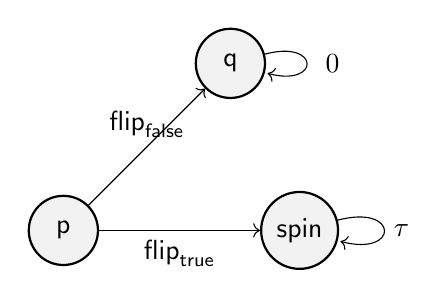
\begin{tikzpicture}
    \node[state] (1) {$\mathsf{q}$};
    \node[state, below left of=1] (2) {$\mathsf{p}$};
    \node[state, right of=2] (3) {$\mathsf{spin}$};
    \draw (2) edge[above] node{$\mathsf{flip}_{\mathsf{false}}$} (1)
    (3) edge[loop right] node{$\tau$} (3)
    (1) edge[loop right] node{$\OUTPUT~0$} (1)
    (2) edge[below] node{$\mathsf{flip}_{\mathsf{true}}$} (3);
  \end{tikzpicture}
  \caption{reifiers are the same}
\end{figure}

\begin{figure}
  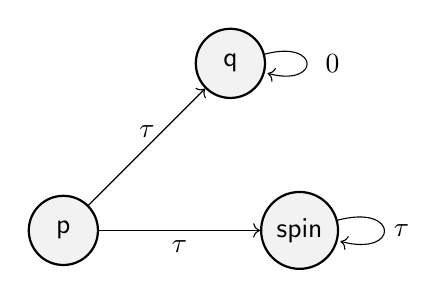
\begin{tikzpicture}
    \node[state] (1) {$\mathsf{q}$};
    \node[state, below left of=1] (2) {$\mathsf{p}$};
    \node[state, right of=2] (3) {$\mathsf{spin}$};
    \draw (2) edge[above] node{$\tau$} (1)
    (3) edge[loop right] node{$\tau$} (3)
    (1) edge[loop right] node{$\OUTPUT~0$} (1)
    (2) edge[below] node{$\tau$} (3);
  \end{tikzpicture}
  \caption{some effects can be marked as hidden}
\end{figure}

\begin{figure}
  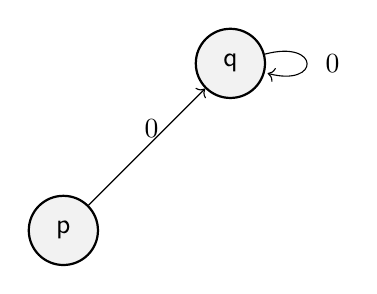
\begin{tikzpicture}
    \node[state] (1) {$\mathsf{q}$};
    \node[state, below left of=1] (2) {$\mathsf{p}$};
    \draw (2) edge[above] node{$\OUTPUT~0$} (1)
    (1) edge[loop right] node{$\OUTPUT~0$} (1);
  \end{tikzpicture}
  \caption{wip}
\end{figure}

%%% Local Variables:
%%% mode: latex
%%% TeX-master: "../main"
%%% End:


% \section{Gitrees in topos of trees}
% \label{global:sec:tot}
% Our goal is to define a weak bisimularity relation of top of guarded
interaction trees. However, there is a subtlety that prevents us from
that. Consider a relation defined by guarded recursion.

\begin{align*}
\end{align*}

But now, if we unveil semantics of the classical topos of trees,
on top of which Iris is built, we can always find a number, for
which that fixpoint relates any guarded interaction tree to
the `bottom' tree defined as $\MU a \col \latert \IT. \Tau(a)$.
Indeed, for a given $n$ that forces the formula, consider instantiating
the existential with $n + 1$. Now, the relation trivially holds, as after
`stripping' $n$ laters, we end up with a proposition that trivially holds.

If we instead consider Transfinite Iris that is meant by allowing us to
force formulas using elements from sets with bigger cardinalities, we
could resolve the problem. However, in this case we lose ability
to define guarded interaction trees as a solution to the recursive domain
equation. Hand-waving proof: the solution to a general recursive domain equation,
given by a locally contractive functor $F \col \ftrcat{\COFEs~\opCat \times \COFEs}{\COFEs}$ with a given element of $F(\One, \One)$ (given by $\One \toby{\mathsf{base}} F(\One, \One)$) is defined as co(limit) of
the following diagram (of type $\ftrcat{\omega}{\COFEs}$).
\begin{align*}
  F_n & \col \COFEs \\
  F_0 & \cceq \One \\
  F_{n + 1} & \cceq F(F_n, F_n) \\
  e_n & \col F_n \toby{} F_{n + 1} \\
  p_n & \col F_{n + 1} \toby{} F_n \\
  e_0 & \cceq \mathsf{base} \\
  e_{n + 1} & \cceq F(p_n, e_n) \\
  p_0 & \cceq \; ! \\
  p_{n + 1} & \cceq F(e_n, p_n)
\end{align*}

\[
  F_0 \stackrel[p_o]{e_0}{\rightleftarrows}
  F_1 \stackrel[p_1]{e_1}{\rightleftarrows}
  \ \cdots \
  \stackrel[p_{n - 1}]{e_{n - 1}}{\rightleftarrows} F_n
\]

It is all nice and cool until we consider if we can take a limit of
$F_n$. Consider an arbitrary equalizing pair of arrows in $\COFEs$:
\parpair{X}{Y}{f}{g}. We want to find a unique ($E \col \COFEs$, $E
\toby{e} X$), s.t. $\forall x \col E. f(e(x)) \equiv g(e(x))$. In a
transfinite setting, it means that $e$ should be continuous (i.e., $e
(\mathsf{blim}_{\leftarrow \beta_i})$ should be preserved), however,
we have no guarantees that $E$, formed as a set-based equalizer, has all
bounded limits.

We argue that working in $\psh{\lambda}$, where $\lambda$ --- an
arbitrary limit ordinal, is enough and sufficient for our goal. First,
sheaf condition (which we need for fixpoints) for $F \col
\psh{\lambda}$ is simple to handle:
\begin{align*} F(\lt{\beta_i}) \equiv \lt{F(\beta_i)}
\end{align*}

Second, the notion of distance and local contractivity scales well
for $\lambda$-indexed (pre)sheaves. Let us debacle it.
Classically, $F$ is contractive, if $\Exists G. F \equiv G \circ \Next$.
\begin{align*}
  \latert & \col \psh{\lambda} \rightarrow \psh{\lambda} \\
  \latert~X~0 & \cceq \One \\
  \latert~X~(n + 1) & \cceq X~n \\
  \latert~X~(\lt{\beta_i}) & \cceq X~(\lt{\beta_i})
\end{align*}
\begin{align*}
  \Next & \col X \rightarrow \latert X \\
  \Next_o & \cceq \; ! \\
  \Next_{n + 1} & \cceq \mathsf{restr}^{n + 1}_{n} \\
  \Next_{\lt{\beta_i}} & \cceq \imath
\end{align*}

We define $x \stackrel{n}{\equiv} y \cceq \All (n \toby{\delta} n'). x(n') \equiv y(n')$.
$F$ is contractive iff $x \stackrel{n}{\equiv} y \implies F(x) \stackrel{n + 1}{\equiv} F(y)$.
Let us show that our notion of being contractive is sufficient:
$(\All (n' < n). x(n') \equiv y(n')) \implies (\All (n' < n + 1). G(\Next(x))(n') \equiv G(\Next(y))(n'))$. We show it by induction on $n'$.
% \begin{itemize}
%   \item[$n' = 0$.] $G(\star) \equiv G(\star)$.
%   \item[$n' = n'' + 1$.] Ists.
%   \item[$\lt{\beta_i}$.]
% \end{itemize}

What is done:
\begin{itemize}
\item Cartesian close structure of $\psh{\cat{C}}$.
\item Completeness and cocompleteness of $\psh{\cat{C}}$.
\item Wrappers around Kripke-Joyal semantics for $\psh{\cat{C}}$ that
we intend to use as internal language.
\item $\latert$, $\later$, $\Next$ for $\psh{\omega}$, including
fixpoints, L\"ob induction.
\item A machinery to piggy-back on Iris framework by using
$\psh{\omega}$ instead of $\COFEs$. (Includes bi-instance for internal logic.)
\item Half-finished solver for recursive domain equations for
$\psh{\omega}$.
\end{itemize}

What remains to be done:
\begin{itemize}
\item Half-finish the solver for recursive domain equations for
$\psh{\omega}$.
\item Port $\psh{\omega}$-specific parts t $\psh{\lambda}$, where
$\lambda$ --- an arbitrary limit ordinal.
\item Port guarded interaction trees to $\psh{\lambda}$.
\end{itemize}

What are some open problems:
\begin{itemize}
\item What flavor of ordinals we should use? Ideally, it should have
good induction scheme.
\end{itemize}

% \begin{tikzcd}
%   A \arrow[d, "g"] \arrow[r, "f"] & B \arrow[r, "\alpha"] \arrow[d, "\gamma"] & D \arrow[d, "\beta"] \\
%   C \arrow[rru, "h"] & B' \arrow[r, "\lambda"] & D'
% \end{tikzcd}

%%% Local Variables:
%%% mode: latex
%%% TeX-master: "../main"
%%% End:


\nocite{*}
\bibliography{refs}

\end{document}
\endinput

%%% Local Variables:
%%% mode: latex
%%% TeX-master: t
%%% End:
